\documentclass[12pt]{article}
\usepackage[utf8]{inputenc}
\usepackage[margin=1in]{geometry}
\usepackage{tabularx}
\usepackage{booktabs}
\usepackage{hyperref}
\usepackage{graphicx}
\usepackage{amsmath}
\usepackage{amssymb}
\usepackage{float}
\usepackage[table]{xcolor}
\usepackage{colortbl}

\definecolor{clrBaseline}{HTML}{5b9bd5}
\definecolor{clrGreedy}{HTML}{ed7d31}
\definecolor{clrRanked}{HTML}{70ad47}
\definecolor{clrBalancer}{HTML}{ffc000}
\definecolor{clrAll}{HTML}{7030a0}

\begin{document}

\date{14/05/2026r.}

% Title page
\begin{titlepage}
    \centering
    {\includegraphics[width=5cm]{logo-PWr.jpg}}\\[1.5cm]
    {\large Faculty: W4N \\}
    {\large Field of study: Computer Engineering, Master's degree} \\[1cm]
    \hrule
    \vspace{1cm}
    {\Huge \textbf{Optimization Methods: Theory and
Applications\\}}
    \vspace{1cm}
    \hrule
    \vspace{1cm}
    { \textbf{Subject:} \\}
    Max-cut problem with evolutionary algorithm and heuristics \\[3cm]

    \textbf{Authors:} \\
    Wincenty Wensker (272760)\\[0.15cm]
    Vadzim Kasyan (294503)\\[0.15cm]
    Kostiantyn Slobodnyi (294498)\\[1cm]
    
    \textbf{Date:} \\
    14.05.2026r.
\end{titlepage}
\newpage
\tableofcontents
\newpage

% ─────────────────────────────────────────────────────────────────────────────
\section{Problem Description}
 
The Max-Cut problem is a classical combinatorial optimization problem.
Given an undirected graph $G = (V, E)$ with edge weights $w : E \to \mathbb{R}^+$,
the goal is to divide the vertex set $V$ into two disjoint subsets such that the total
weight of edges running between them is as large as possible.
 
The problem is NP-hard, making exact solutions infeasible for large graphs.
Practical approaches therefore rely on approximation algorithms or metaheuristics;
in this project, an evolutionary algorithm is used.
 
% ─────────────────────────────────────────────────────────────────────────────
\section{What We Optimize}
 
\subsection{Objective Function}
 
Let $S \subseteq V$ denote one side of the partition, with the other side being
$V \setminus S$. The quantity being maximized is the total weight of edges whose
endpoints lie in different parts of the partition:
 
\begin{equation}
    f(S) \;=\; \sum_{\substack{(u,v)\,\in\, E \\ u \in S,\; v \notin S}} w(u, v)
    \label{eq:cut}
\end{equation}
 
The optimal solution is $S^* = \arg\max_{S \subseteq V} f(S)$.
For unweighted graphs ($w \equiv 1$) this reduces to maximizing the number of
crossing edges.
 
\subsection{Practical Evaluation}
 
Computing $f(S)$ for a given assignment requires a single iteration over all edges,
checking whether the two endpoints belong to different parts. This is $O(|E|)$ per
evaluation, which remains efficient even for graphs with thousands of edges.
 
% ─────────────────────────────────────────────────────────────────────────────
\section{Solution Encoding}
\label{sec:encoding}
 
\subsection{Encoding Type}
 
The chosen encoding is binary. Each candidate solution is a vector
$x \in \{0, 1\}^{|V|}$ where the $i$-th bit indicates partition membership of
vertex $i$:
 
\begin{equation}
    x[i] = \begin{cases} 1 & \text{if vertex } i \in S \\ 0 & \text{if vertex } i \notin S \end{cases}
\end{equation}
 
This is the natural choice for Max-Cut because the decision space is inherently binary, since every vertex belongs to exactly one of the two partitions.
The chromosome length equals $|V|$, and the search space contains $2^{|V|}$ possible
solutions (effectively $2^{|V|-1}$ unique cuts due to the symmetry discussed below).
 
\subsection{Genetic Operators}
 
\begin{itemize}
    \item Mutation: Bit-flip with probability $p_m = 1/|V|$, yielding one
          expected change per individual per generation.
    \item Crossover: Single-point or uniform crossover, both directly applicable
          without any repair step since every binary string represents a valid partition.
\end{itemize}
 
\subsection{Symmetry}
 
The encoding is symmetric: any solution $x$ and its complement $\bar{x}$ represent
the same cut with the same value. To reduce this redundancy, vertex~0 can be fixed to
partition $S$ (i.e.\ $x[0] = 0$ always), halving the effective search space.
 
% ─────────────────────────────────────────────────────────────────────────────
\section{Problem Instances}

All nine instances are drawn from the Biq Mac Library~\cite{biqmac}, a dedicated
collection of Max-Cut and binary quadratic programming benchmarks maintained by
Angelika Wiegele at Alpen-Adria-Universität Klagenfurt.
The library is the standard reference for testing exact and heuristic Max-Cut solvers. Instances are grouped into families distinguished by graph topology, edge density,
and weight scheme, which together determine the hardness and character of the
resulting optimisation landscape.

\subsection{File Format}

Every instance in the Biq Mac Library is stored in the \emph{rudy} output format,
named after the graph generator tool used to produce the instances~\cite{rudy}.
The format is a plain-text edge list:

\begin{verbatim}
n   m
h_1 t_1 c_{h_1,t_1}
h_2 t_2 c_{h_2,t_2}
...
h_m t_m c_{h_m,t_m}
\end{verbatim}

\noindent
The first line contains two integers: $n$ (number of vertices) and $m$ (number of
edges). Each of the following $m$ lines describes one undirected edge: $h_i$ and
$t_i$ are the one-based indices of the two endpoints, and $c_{h_i,t_i}$ is the
integer edge weight. Because each edge is listed exactly once, the full symmetric
adjacency is reconstructed during loading by treating every entry as bidirectional.

\subsection{Instance Families}

\subsubsection*{g05: Unweighted Random Graphs}

Instances of the form \texttt{g05\_n.i} are unweighted Erd\H{o}s--R\'enyi random
graphs with $n$ vertices and edge probability $0.5$, generated by rudy.
All edge weights are $1$; the objective reduces to maximising the number of crossing
edges.
The uniform structure and moderate density make these good baseline instances: the
landscape is relatively smooth, local optima are plentiful but shallow, and the
optimal cut value scales predictably with $n$.

\begin{itemize}
    \item \texttt{g05\_60.1} ($n=60$, $m\approx885$): smallest instance in the
          suite, used for rapid correctness checks and convergence profiling.
    \item \texttt{g05\_80.1} ($n=80$, $m\approx1580$): same family at larger
          scale, exposing how the algorithm handles the increased search space
          $2^{79}$ while the landscape character remains the same.
\end{itemize}

\subsubsection*{pm1s / pm1d: Sparse and Dense Frustrated Graphs}

Instances of the form \texttt{pm1s\_n.i} (sparse, density~0.1) and
\texttt{pm1d\_n.i} (dense, density~0.99) have integer edge weights drawn uniformly
from $\{-1, 0, +1\}$.
The presence of negative weights introduces \emph{frustration}: satisfying one edge
(placing its endpoints in different partitions) forces the violation of a
negatively-weighted edge elsewhere.
This creates a rugged landscape with exponentially many local optima, making these
instances significantly harder than the unweighted \texttt{g05} family of the same
size.

\begin{itemize}
    \item \texttt{pm1s\_100.1} ($n=100$, $m\approx990$): sparse frustrated
          graph. Low density means the graph is nearly forest-like in places;
          negative weights cluster around a small fraction of edges, creating
          isolated pockets of frustration.
    \item \texttt{pm1d\_100.9} ($n=100$, $m\approx9900$): near-complete graph
          with frustrated weights. The density is the dominant challenge here:
          almost every pair of vertices is connected, so every partition decision
          has global consequences. This is the hardest instance among those with
          $n=100$.
\end{itemize}

\subsubsection*{w / pw: Integer-Weighted Random Graphs}

Instances of the form \texttt{wd\_100.i} have integer weights drawn from
$[-10, 10]$, while \texttt{pwd\_100.i} restricts weights to $[1, 10]$ (positive
only).
The wider weight range relative to the \texttt{pm1} family means individual edges
differ substantially in importance, so the objective landscape is more varied and
greedy decisions based on single-edge gain are more informative.

\begin{itemize}
    \item \texttt{w01\_100.1} ($n=100$, density~0.1, weights~$[-10,10]$):
          sparse graph with signed wide-range weights. The combination of low
          density and large negative weights produces deep, narrow local optima.
    \item \texttt{w09\_100.9} ($n=100$, density~0.9, weights~$[-10,10]$):
          dense counterpart. Near-complete connectivity with wide signed weights;
          the benchmark role here is analogous to \texttt{pm1d} but with a richer
          weight distribution that stresses weight-aware operators.
    \item \texttt{pw09\_100.9} ($n=100$, density~0.9, weights~$[1,10]$):
          positive-only wide weights at high density. Because no negative weights
          are present, frustration is absent and the landscape is smoother than
          \texttt{w09}. The contrast between this instance and \texttt{w09\_100.9}
          isolates the effect of negative weights on algorithm performance.
\end{itemize}

\subsubsection*{t2g: Two-Dimensional Toroidal Ising Spin Glasses}

Instances of the form \texttt{t2gn\_seed} are two-dimensional toroidal grid graphs
of size $\sqrt{n} \times \sqrt{n}$ (so $n$ is a perfect square) with
Gaussian-distributed real-valued edge weights, generated following the statistical
physics model of Frauke Liers~\cite{liers}.
Each vertex is connected to its four grid neighbours (up, down, left, right) with
wrap-around boundary conditions, giving exactly $m = 2n$ edges.
The Gaussian weights can be positive or negative, yielding frustrated cycles that
are the defining feature of the \emph{Ising spin glass} model.
The highly regular topology combined with frustration makes these instances
notoriously difficult for local search: the energy landscape has exponentially many
near-degenerate local optima and the graph diameter is small, so perturbations
propagate quickly.

\begin{itemize}
    \item \texttt{t2g10\_5555} ($n=100$, $m=200$, seed \texttt{5555}): $10\times10$
          toroidal Ising instance. Despite having only 200 edges, this instance
          is harder than any of the \texttt{g05} or \texttt{pm1s} instances at
          $n=100$ because of the structured frustration inherent to the spin-glass
          topology. Used to evaluate how the algorithm behaves on highly structured
          graphs with a rugged, correlated landscape.
    \item \texttt{t2g10\_6666} ($n=100$, $m=200$, seed \texttt{6666}): identical
          topology and weight distribution, different random seed. Including two
          instances from the same family with different seeds allows assessment of
          landscape sensitivity: if algorithm performance varies substantially
          between \texttt{t2g10\_5555} and \texttt{t2g10\_6666}, the heuristic is
          sensitive to the specific realisation of the disorder rather than robustly
          solving the spin-glass structure.
\end{itemize}

\subsection{Summary Table}

\begin{table}[H]
    \centering
    \begin{tabularx}{\textwidth}{|l|l|X|X|X|X|}
        \hline
        \textbf{Instance} & \textbf{Family} & $|V|$ & $|E|$ & \textbf{Weights} & \textbf{Key trait} \\
        \hline
        \texttt{g05\_60.1}   & g05  & 60  & $\approx$885   & $\{0,1\}$      & Unweighted, baseline \\
        \hline
        \texttt{g05\_80.1}   & g05  & 80  & $\approx$1580  & $\{0,1\}$      & Unweighted, scaling \\
        \hline
        \texttt{pm1s\_100.1} & pm1s & 100 & $\approx$990   & $\{-1,0,1\}$   & Sparse, frustrated \\
        \hline
        \texttt{pm1d\_100.9} & pm1d & 100 & $\approx$9900  & $\{-1,0,1\}$   & Dense, heavy frustration \\
        \hline
        \texttt{w01\_100.1}  & w    & 100 & $\approx$990   & $[-10,10]$     & Sparse, wide signed weights \\
        \hline
        \texttt{w09\_100.9}  & w    & 100 & $\approx$9900  & $[-10,10]$     & Dense, wide signed weights \\
        \hline
        \texttt{pw09\_100.9} & pw   & 100 & $\approx$9900  & $[1,10]$       & Dense, positive-only weights \\
        \hline
        \texttt{t2g10\_5555} & t2g  & 100 & 200            & Gaussian       & 2D torus Ising spin-glass \\
        \hline
        \texttt{t2g10\_6666} & t2g  & 100 & 200            & Gaussian       & Same topology, different seed \\
        \hline
    \end{tabularx}
    \caption{Summary of the nine benchmark instances from the Biq Mac Library.
             The three instances intended for primary benchmarking are
             \texttt{pm1d\_100.9}, \texttt{w09\_100.9}, and \texttt{pw09\_100.9},
             as their near-complete graphs represent the most demanding workload
             in the collection.}
    \label{tab:instances}
\end{table}

% ─────────────────────────────────────────────────────────────────────────────
\section{Baseline Genetic Algorithm}
\label{sec:baseline}

Before introducing problem-specific heuristics it is necessary to establish a
reference implementation: a genetic algorithm that uses only standard, well-studied
components with no domain knowledge built in.
All performance comparisons in this project measure improvement relative to this
baseline, so its design choices must be well-justified and representative of
mainstream practice.

\subsection{Algorithm Outline}

The algorithm follows the canonical generational GA loop.
An initial population of $\mu$ individuals is created by assigning each gene
independently and uniformly at random, with vertex~0 fixed to partition $S$
throughout (see Section~\ref{sec:encoding}).
Each individual is evaluated once immediately after creation.
The loop then repeats until the fitness function evaluation budget is exhausted:
a new population of size $\mu$ is assembled from the current one, the current
population is discarded, and the new population takes its place.
The best individual ever seen across all generations is tracked separately and
returned as the final answer.

\subsection{Selection}

Parent selection uses \emph{tournament selection} with tournament size $k = 3$.
Three individuals are drawn uniformly at random from the population (with
replacement) and the one with the highest fitness wins the tournament and is
used as a parent.
The process is repeated independently to obtain the second parent.

Tournament selection was chosen over fitness-proportionate (roulette-wheel)
selection for two reasons.
First, it is robust to fitness scaling issues: it depends only on the relative
ordering of fitness values within each tournament, not on their absolute magnitudes
or ratios.
This is important for Max-Cut instances where the range of cut values can vary by
orders of magnitude across instance families.
Second, the selection pressure is easily controlled by the tournament size $k$:
larger $k$ increases pressure (the best individual wins more often), smaller $k$
reduces it.
The value $k = 3$ is the most common default in the literature, providing moderate
pressure without converging prematurely.

\subsection{Crossover}

Offspring are produced by \emph{uniform crossover} applied with probability
$p_c = 0.8$.
Each gene of the offspring is inherited from parent~A or parent~B with equal
probability, independently for every position.
If crossover is not applied (probability $1 - p_c = 0.2$), the offspring is an
unmodified copy of parent~A.

Uniform crossover was preferred over single-point or two-point crossover because
it does not impose any positional bias: there is no notion of a ``building block''
region defined by chromosomal proximity, which is particularly appropriate here
since the vertex indices are arbitrary labels with no inherent spatial relationship.
For Max-Cut on general graphs, vertices that are functionally related (connected by
heavy edges) are not necessarily adjacent in the chromosome, so crossover operators
that respect positional locality offer no structural benefit and may actively
fragment meaningful partial solutions.
The crossover rate of $0.8$ is the standard default used in the majority of GA
studies and represents a strong but not exclusive preference for recombination over
cloning.

\subsection{Mutation}

After crossover, every gene in the offspring is independently subjected to
\emph{bit-flip mutation}: the gene is inverted with probability

\begin{equation}
    p_m \;=\; \frac{1}{|V|}
\end{equation}

This yields an expected number of exactly one flip per offspring per generation,
regardless of chromosome length.
The $1/|V|$ rule is the canonical default for binary GAs and has a solid theoretical
basis: with smaller rates the algorithm explores too slowly, while with larger rates
the search degrades toward random walk.
Vertex~0 is never flipped, consistent with the symmetry convention.

\subsection{Elitism}

The two fittest individuals from the current generation are copied directly into
the next population without modification (\emph{elitism count} $= 2$).
The remaining $\mu - 2$ slots are filled by offspring from crossover and mutation.
Elitism guarantees that the best solution found so far is never lost to random
variation, which stabilises convergence and prevents regression.
Two elites rather than one are retained to preserve a small amount of genetic
diversity at the top of the fitness ranking while still providing strong protection
against fitness loss.

\subsection{Termination Criterion}

The algorithm terminates when the total number of fitness function evaluations
reaches a fixed \emph{budget} $B$ (default $B = 50{,}000$).
The budget is enforced at the level of individual offspring: generation boundaries
are not synchronisation points, and the loop exits as soon as the counter reaches
$B$ even if the current generation is not complete.

A fixed evaluation budget was chosen as the termination criterion in preference to
a fixed generation count because it provides a fair basis for comparison between
algorithms with different population sizes or offspring counts.
Two algorithms that both consume 50{,}000 evaluations have spent the same
computational effort on the objective function, regardless of how they internally
structured that effort into generations.
This is the standard approach in algorithm benchmarking studies, in particular on
the BBOB/COCO platform.
A fixed generation count, by contrast, conflates the number of generations with
the cost per generation, making cross-algorithm comparisons ambiguous.

\subsection{Configuration Summary}

\begin{table}[H]
    \centering
    \begin{tabularx}{0.75\textwidth}{|l|X|}
        \toprule
        \textbf{Parameter} & \textbf{Value} \\
        \midrule
        Population size $\mu$       & 100 \\
        NFE budget $B$              & 50{,}000 \\
        Selection                   & Tournament, $k = 3$ \\
        Crossover                   & Uniform, $p_c = 0.8$ \\
        Mutation                    & Bit-flip, $p_m = 1/|V|$ \\
        Elitism                     & 2 individuals \\
        Initialisation              & Uniform random (vertex~0 fixed to 0) \\
        \bottomrule
    \end{tabularx}
    \caption{Parameter configuration of the baseline genetic algorithm.
             All three metaheuristic enhancements are disabled in this configuration.}
    \label{tab:baseline}
\end{table}

\subsection{Rationale as a Baseline}

The configuration above was deliberately constructed to be \emph{generic}: no
parameter depends on the structure of the graph, the weight distribution, or any
property of the specific instance being solved.
Every component (tournament selection, uniform crossover, $1/|V|$ bit-flip mutation,
two-elite replacement) is a well-established default that appears in textbook
treatments of genetic algorithms~\cite{dejong,goldberg} and is representative of
what a practitioner would implement without any domain knowledge.

This genericity is precisely what makes it a useful baseline.
Any improvement demonstrated by the metaheuristic enhancements described in
Section~\ref{sec:metaheuristics} is unambiguously attributable to the exploitation
of problem structure, since the underlying algorithm, the evaluation budget, and
all other parameters remain identical.
A more sophisticated baseline, for instance one using adaptive parameter control or
a problem-specific repair operator by default, would make it harder to isolate the
contribution of each individual enhancement.

The choice of $\mu = 100$ and $B = 50{,}000$ yields approximately $500$ full
generations for the default configuration, which is sufficient for convergence on
the benchmark instances used while keeping wall-clock time well under one second
per run.
This allows large numbers of repeated trials to be conducted efficiently, which is
important given the stochastic nature of the algorithm.

% ─────────────────────────────────────────────────────────────────────────────
\section{Metaheuristic Enhancements}
\label{sec:metaheuristics}

The baseline evolutionary algorithm described in Section~\ref{sec:baseline} operates
with a uniform crossover, a flat bit-flip mutation, and purely random initialisation.
While this constitutes a sound and reproducible reference point, the algorithm makes
no use of problem structure: every vertex is treated identically regardless of how
influential it is in the graph, and every offspring is allowed to deviate arbitrarily
from any notion of a well-formed partition.
The three enhancements described in this section each address a distinct weakness of
the baseline and are designed to compose with one another without conflict.
All three are optional and controlled by configuration parameters, so the baseline
behaviour is recovered exactly when all enhancements are disabled.

A central concept shared by two of the three mechanisms is a \emph{node ranking}.
Before the evolutionary loop begins, every vertex $v \in V$ is assigned a scalar
importance score equal to the sum of absolute edge weights over all its incident
edges:

\begin{equation}
    \sigma(v) \;=\; \sum_{(v,\,u)\,\in\,E} |w(v, u)|
\end{equation}

Vertices are then sorted in descending order of $\sigma$, producing a static ranking
$v_{(1)}, v_{(2)}, \ldots, v_{(|V|)}$ where $v_{(1)}$ is the most influential vertex
and $v_{(|V|)}$ the least.
This ranking is computed once at startup and re-used throughout the run, so its cost
is negligible.
Its purpose is to provide a principled, domain-aware notion of vertex importance that
the heuristic operators can exploit.

\subsection{Greedy-by-Node Repair}
\label{sec:greedy-repair}

The greedy-by-node repair mechanism addresses the fact that the baseline crossover
and mutation operators are oblivious to the structure of the cut.
After crossing two parents, the resulting offspring may assign influential, heavily
connected vertices to whichever partition happened to be inherited, with no regard
for whether that assignment is locally sensible.

The mechanism works in two phases.
In the first phase, carried out once before the evolutionary loop, a greedy
reference solution is constructed using the node ranking.
Vertices are processed in order of decreasing importance $\sigma(v)$.
For each vertex, the cut contributions of placing it in partition $S$ or $V \setminus S$
are evaluated with respect to all already-assigned neighbours: the vertex is assigned
to whichever side maximises the weight of crossing edges to those neighbours.
If no neighbour has been assigned yet, the vertex receives a random assignment.
Vertex~0 is fixed to $S$ throughout, consistent with the symmetry convention
described in Section~\ref{sec:encoding}.
The result is a single greedy partition $x^{g}$ that respects the importance ordering
and serves as a structural reference.

In the second phase, during offspring generation, a fraction $r$ of offspring
(configurable, default $0.5$) are subjected to repair after crossover and before
mutation.
Repair overwrites the genes of the top $\lceil \alpha \cdot |V| \rceil$ vertices in
the ranking (default $\alpha = 0.2$, i.e.\ the top 20\,\%) with the values from
$x^{g}$, leaving the remaining genes untouched.
Mutation is then applied to the repaired offspring, allowing the lower-ranked genes
to continue evolving freely while the core partition structure imposed by the greedy
solution is preserved.

The rationale is that the most influential vertices dominate the cut value.
Fixing their assignments to a greedy optimum reduces the effective search space to
the lower-ranked, less critical vertices, where the evolutionary operators have the
greatest relative freedom and where random variation causes the least structural
damage.
This is a form of problem decomposition guided by domain knowledge rather than
random sampling.

\subsection{Ranked Mutation}
\label{sec:ranked-mutation}

The standard bit-flip mutation applies the same probability $p_m = 1/|V|$ to every
vertex.
This is appropriate when all vertices are equally important, but in Max-Cut the
importance distribution is highly skewed: a small number of high-degree, high-weight
vertices account for a disproportionate share of the objective value, while the
majority of vertices have limited influence.
Applying the same mutation pressure to a hub vertex as to a peripheral leaf is
wasteful at best and destructive at worst.

The ranked mutation operator replaces the uniform rate with a per-vertex rate derived
from the node ranking.
The rate for vertex $v$ at rank $k$ (where rank $1$ is most important) is computed
by linear interpolation between a minimum multiplier $\mu_{\min}$ and a maximum
multiplier $\mu_{\max}$:

\begin{equation}
    p_m(v_{(k)}) \;=\; p_m^{\text{base}} \cdot
    \left( \mu_{\min} + \frac{k-1}{|V|-1}\,(\mu_{\max} - \mu_{\min}) \right)
\end{equation}

The top-ranked vertex receives rate $p_m^{\text{base}} \cdot \mu_{\min}$ and the
bottom-ranked vertex receives $p_m^{\text{base}} \cdot \mu_{\max}$.
With default values $\mu_{\min} = 0.25$ and $\mu_{\max} = 2.0$, the most influential
vertex is mutated at one quarter of the base rate and the least influential vertex at
twice the base rate, an eight-fold spread across the ranking.

Optionally, the per-vertex rates can be normalised so that their mean equals
$p_m^{\text{base}}$, preserving the expected number of flips per offspring at
approximately one.
Normalisation ensures that the ranked and flat mutation operators consume the same
average mutation budget, making any performance difference attributable purely to
the redistribution of mutation pressure rather than to a change in overall mutation
intensity.
When normalisation is disabled, the operator instead applies strictly more mutation
pressure to low-ranked vertices and less to high-ranked ones, at the cost of making
the comparison with the baseline less direct.

The mechanism is complementary to the greedy-by-node repair: repair fixes the top
vertices to a greedy reference, while ranked mutation suppresses random perturbation
of those same vertices and concentrates exploratory variation on the periphery of
the ranking where it is least likely to damage the core partition structure.

\subsection{Balancer}
\label{sec:balancer}

Neither the baseline operators nor the two mechanisms above impose any constraint on
the size of the two partitions.
Crossover and mutation can freely produce heavily asymmetric solutions in which one
side of the partition contains the vast majority of vertices.
Such solutions are not invalid (every binary string represents a legal partition),
but they are structurally poor: a partition with $|S| \approx 1$ and
$|V \setminus S| \approx |V|$ can cut at most a small fraction of edges by volume,
and the evolutionary dynamics that produced it are unlikely to escape toward more
balanced, higher-quality regions without a structural correction.

The balancer operator corrects excessive imbalance after mutation.
It is parameterised by a target interval $[\beta_{\min},\, \beta_{\max}]$ for the
fraction of vertices assigned to $S$ (default $[0.4, 0.6]$, i.e.\ the
40\,\%--60\,\% band).
After mutation, if $|S| / |V|$ falls within the target interval the operator does
nothing.
If the partition is outside the interval, the operator identifies the larger side and
moves vertices from that side to the other until balance is restored.

The choice of which vertices to flip is not arbitrary.
For each vertex $v$ on the larger side, the operator computes the \emph{local flip
gain}:

\begin{equation}
    g(v) \;=\; \sum_{(v,\,u)\,\in\,E} w(v,u)\cdot\bigl[\,x[u] \neq x[v]\,\bigr]
    \;-\; \sum_{(v,\,u)\,\in\,E} w(v,u)\cdot\bigl[\,x[u] = x[v]\,\bigr]
\end{equation}

That is, $g(v)$ is the net change in cut value that would result from moving $v$
to the other partition, considering only edges incident to $v$.
The operator sorts the candidate vertices by $g(v)$ in descending order and flips
from the bottom of the list: the vertices with the smallest (or most negative) gain
are those contributing least to the cut in their current position and are therefore
the least costly to move.
Vertex~0 is never flipped, preserving the symmetry convention.

This greedy selection strategy ensures that the rebalancing step causes as little
damage to the objective as possible.
Unlike the greedy-by-node repair, which enforces a specific partition structure, the
balancer makes only the minimum number of targeted changes needed to restore
dimensional feasibility, and does so in a locally optimal order.
Fitness is evaluated once after all three operators (repair, ranked mutation,
balancer) have been applied, so the balancer incurs no additional objective function
calls.

% ─────────────────────────────────────────────────────────────────────────────
\section{Testing Methodology}
\label{sec:testing}

\subsection{Objectives and Scope}

The purpose of the experimental evaluation is to compare the performance of the
baseline genetic algorithm (Section~\ref{sec:baseline}) against each of the three
metaheuristic enhancements (Section~\ref{sec:metaheuristics}), both individually
and in combination.
Because the algorithm is stochastic, a single run carries no statistical meaning;
repeated trials are required to obtain reliable estimates of central tendency and
variance for each configuration.

The evaluation is structured around two questions.
First, does each individual enhancement improve upon the baseline on the instance
families for which it was designed?
Second, does combining all three enhancements simultaneously yield further
improvement over any single enhancement, or does the interaction between them
introduce interference that reduces the benefit of each component?

\subsection{Test Matrix}

Every combination of instance and configuration is treated as an independent
experiment.
The full test matrix is as follows:

\begin{itemize}
    \item \textbf{Standard experiments}: all nine benchmark instances crossed with
          four configurations (baseline, greedy-by-node only, ranked mutation
          only, and balancer only), each repeated \textbf{5 times}.
          This yields $9 \times 4 \times 5 = 180$ runs and allows the isolated
          effect of each heuristic to be measured across the full range of instance
          families.
    \item \textbf{Primary experiments}: the three hardest instances
          (\texttt{pm1d\_100.9}, \texttt{w09\_100.9}, \texttt{pw09\_100.9}) with
          all three heuristics enabled simultaneously, each repeated
          \textbf{10 times}.
          This yields $3 \times 10 = 30$ runs and provides a higher-confidence
          estimate of the combined configuration on the instances where
          improvement is expected to be most visible.
\end{itemize}

The total number of runs is 210.
All five configurations for the primary instances are therefore available for
comparison: baseline, each single heuristic at 5 runs, and the combined
configuration at 10 runs.

\subsection{Test Automation}

All experiments are executed by a dedicated Python script (\texttt{run\_tests.py})
that drives the compiled C++ binary (\texttt{ga\_main}) as a subprocess.
The binary is invoked with the \texttt{--json} flag, which suppresses the
human-readable console output and instead emits a single JSON object per run
on standard output.
This eliminates any text-parsing ambiguity and allows the runner to ingest results
directly via the standard library JSON parser with no post-processing.

For each run the script records: the instance file, the configuration file, the
active heuristic flags, the best cut value found, the total number of fitness
function evaluations consumed, the number of complete generations executed, the
wall-clock time of the evolutionary loop in milliseconds, the stop reason, and the
full best-solution vector.
After all runs complete, the script writes three output files:

\begin{itemize}
    \item \texttt{results/raw.jsonl}: one JSON record per run in newline-delimited
          format, containing all of the above fields including the complete
          solution vector.
          This file is the primary archival record and can be loaded directly
          into data-analysis tools such as pandas.
    \item \texttt{results/summary.csv}: one row per (instance, configuration)
          pair with aggregate statistics (best, worst, mean, standard deviation of
          cut value; mean and standard deviation of wall-clock time; mean NFE and
          generation count).
    \item \texttt{results/report.txt}: a human-readable formatted table
          identical in content to the CSV but intended for direct reading.
\end{itemize}

\subsection{Measured Metrics}

The following quantities are recorded for every run and used in the analysis.

\paragraph{Best cut value.}
The primary performance metric is $f^* = \max_t f(x_t)$, the highest cut value
found by the algorithm across all generations in a single run.
This is the quantity the algorithm directly optimises and is the natural basis for
comparing solution quality across configurations.

\paragraph{Mean and standard deviation of cut value.}
Aggregated over repeated runs, the mean $\bar{f}^*$ measures the expected solution
quality and the standard deviation $\sigma_{f^*}$ measures consistency.
A configuration with a high mean but also a high standard deviation performs well
on average but is unreliable; a configuration with a lower mean but near-zero
standard deviation is more predictable.
Both quantities are needed to assess practical usefulness.

\paragraph{Number of fitness function evaluations (NFE).}
All configurations share the same budget $B = 50{,}000$ evaluations and the
termination criterion is the budget exhaustion (see Section~\ref{sec:baseline}).
The NFE reported per run is therefore always equal to $B$ under normal operation,
and its inclusion in the output primarily serves as a consistency check.
In future experiments with early-stopping criteria, the NFE would become a
meaningful variable quantity.

\paragraph{Wall-clock time.}
The elapsed time of the evolutionary loop is measured in milliseconds using a
high-resolution monotonic clock.
It is reported per run and aggregated as mean and standard deviation.
Wall-clock time reflects the combined cost of fitness evaluations, selection,
crossover, mutation, and any heuristic repair operations.
Because the NFE budget is fixed, differences in wall-clock time between
configurations directly quantify the computational overhead introduced by each
metaheuristic enhancement.

\paragraph{Number of generations.}
The number of complete generations executed within the NFE budget depends on the
population size, the elitism count, and whether any per-generation offspring are
skipped when the budget is exhausted mid-generation.
It is recorded primarily to confirm that all configurations exercise a comparable
number of evolutionary cycles.

\subsection{Experimental Platform}

All experiments were conducted on a single machine with no other user workloads
active during the test runs.
Effort was made to minimise interference from background operating system
processes: no interactive applications were running during the experiments and the
machine had been in continuous operation for several days prior, ensuring that any
OS caching and memory management effects had stabilised.

\begin{table}[H]
    \centering
    \begin{tabularx}{0.75\textwidth}{|l|X|}
        \toprule
        \textbf{Property} & \textbf{Value} \\
        \midrule
        Model           & Apple Macbook Pro 14" \\
        Operating system & macOS 26.5.1 (arm64) \\
        Kernel          & Darwin 25.5.0 \\
        CPU             & Apple M4 Pro \\
        Memory          & 24{,}576~MiB (24~GB unified) \\
        Compiler        & \texttt{g++} with \texttt{-std=c++17 -O2} \\
        Python          & CPython 3.14 (test runner only) \\
        \bottomrule
    \end{tabularx}
    \caption{Hardware and software configuration of the experimental platform.}
    \label{tab:platform}
\end{table}

\noindent
The Apple M4 Pro is an ARM-based system-on-chip with a unified memory architecture.
The binary was compiled natively for arm64 with full optimisation (\texttt{-O2})
and no architecture-specific tuning flags beyond the toolchain defaults.
Because the algorithm is single-threaded, the number of performance cores available
is not relevant; the results reflect single-core throughput only.
The 210 runs of the full test matrix completed in approximately 22 seconds of
wall-clock time, with individual runs averaging 65--80~ms each depending on the
instance and configuration.

\subsection{Reproducibility}

The random seed is set via the operating system random device (\texttt{/dev/urandom})
independently for each run, meaning that repeated invocations of the test script
will produce different specific solutions but statistically equivalent distributions.
To reproduce exact numerical results, a fixed seed can be set via the
\texttt{random\_seed} parameter in the configuration file.
The full solution vector for every run is stored in \texttt{results/raw.jsonl},
which allows any individual result to be inspected or re-evaluated offline.

% ─────────────────────────────────────────────────────────────────────────────
\section{Results}
\label{sec:results}

\subsection{Overview}

This section presents the numerical results of the 210-run benchmark described
in Section~\ref{sec:testing}.
All runs used the same NFE budget of $B = 50{,}000$ and the parameter defaults
from Table~\ref{tab:baseline}.
Results are organised into two parts: a complete numerical tables covering all
nine instances and all configurations, followed by three figures that visualise
the patterns across instance families.

\subsection{Complete Results Tables}

Tables~\ref{tab:results-g05}--\ref{tab:results-t2g} report, for every
(instance, configuration) pair, the best cut value found across all runs, the
mean and standard deviation of the cut value, and the mean wall-clock time of
the evolutionary loop.
Configurations are listed in the order: baseline, greedy-by-node, ranked
mutation, balancer, and (for primary instances) all three combined.

% ── g05 family ───────────────────────────────────────────────────────────────
\begin{table}[H]
\centering
\begin{tabular}{|l|l|r|r|r|r|}
\toprule
\textbf{Instance} & \textbf{Config} & \textbf{Best} & \textbf{Mean} & \textbf{Std} & \textbf{Time (ms)} \\
\midrule
\texttt{g05\_60.1} & \cellcolor{clrBaseline!25}Baseline    & \cellcolor{clrBaseline!25}528 & \cellcolor{clrBaseline!25}524.4 & \cellcolor{clrBaseline!25}3.3  & \cellcolor{clrBaseline!25}54.3 \\
                   & \cellcolor{clrGreedy!25}Greedy        & \cellcolor{clrGreedy!25}530   & \cellcolor{clrGreedy!25}526.4  & \cellcolor{clrGreedy!25}2.5   & \cellcolor{clrGreedy!25}54.9  \\
                   & \cellcolor{clrRanked!25}Ranked Mut.   & \cellcolor{clrRanked!25}531   & \cellcolor{clrRanked!25}526.0  & \cellcolor{clrRanked!25}4.4   & \cellcolor{clrRanked!25}54.1  \\
                   & \cellcolor{clrBalancer!25}Balancer    & \cellcolor{clrBalancer!25}532 & \cellcolor{clrBalancer!25}528.4 & \cellcolor{clrBalancer!25}5.0 & \cellcolor{clrBalancer!25}54.3 \\
\midrule
\texttt{g05\_80.1} & \cellcolor{clrBaseline!25}Baseline    & \cellcolor{clrBaseline!25}941 & \cellcolor{clrBaseline!25}933.8 & \cellcolor{clrBaseline!25}8.9  & \cellcolor{clrBaseline!25}76.5 \\
                   & \cellcolor{clrGreedy!25}Greedy        & \cellcolor{clrGreedy!25}922   & \cellcolor{clrGreedy!25}914.6  & \cellcolor{clrGreedy!25}5.0   & \cellcolor{clrGreedy!25}77.5  \\
                   & \cellcolor{clrRanked!25}Ranked Mut.   & \cellcolor{clrRanked!25}941   & \cellcolor{clrRanked!25}931.6  & \cellcolor{clrRanked!25}14.2  & \cellcolor{clrRanked!25}77.7  \\
                   & \cellcolor{clrBalancer!25}Balancer    & \cellcolor{clrBalancer!25}941 & \cellcolor{clrBalancer!25}926.8 & \cellcolor{clrBalancer!25}13.2 & \cellcolor{clrBalancer!25}76.7 \\
\bottomrule
\end{tabular}
\caption{Results for the \texttt{g05} family (unweighted random graphs).
         All values are over 5 runs.}
\label{tab:results-g05}
\end{table}

% ── pm1 family ───────────────────────────────────────────────────────────────
\begin{table}[H]
\centering
\begin{tabular}{|l|l|r|r|r|r|}
\toprule
\textbf{Instance} & \textbf{Config} & \textbf{Best} & \textbf{Mean} & \textbf{Std} & \textbf{Time (ms)} \\
\midrule
\texttt{pm1s\_100.1} & \cellcolor{clrBaseline!25}Baseline  & \cellcolor{clrBaseline!25}125 & \cellcolor{clrBaseline!25}117.0 & \cellcolor{clrBaseline!25}5.3  & \cellcolor{clrBaseline!25}69.5  \\
                     & \cellcolor{clrGreedy!25}Greedy      & \cellcolor{clrGreedy!25}121   & \cellcolor{clrGreedy!25}115.8  & \cellcolor{clrGreedy!25}3.0   & \cellcolor{clrGreedy!25}70.1   \\
                     & \cellcolor{clrRanked!25}Ranked Mut. & \cellcolor{clrRanked!25}123   & \cellcolor{clrRanked!25}120.8  & \cellcolor{clrRanked!25}2.2   & \cellcolor{clrRanked!25}69.2   \\
                     & \cellcolor{clrBalancer!25}Balancer  & \cellcolor{clrBalancer!25}126 & \cellcolor{clrBalancer!25}119.2 & \cellcolor{clrBalancer!25}5.4 & \cellcolor{clrBalancer!25}69.6  \\
\midrule
\texttt{pm1d\_100.9} & \cellcolor{clrBaseline!25}Baseline  & \cellcolor{clrBaseline!25}405 & \cellcolor{clrBaseline!25}372.2 & \cellcolor{clrBaseline!25}18.5 & \cellcolor{clrBaseline!25}145.7 \\
                     & \cellcolor{clrGreedy!25}Greedy      & \cellcolor{clrGreedy!25}399   & \cellcolor{clrGreedy!25}383.6  & \cellcolor{clrGreedy!25}12.9  & \cellcolor{clrGreedy!25}146.5  \\
                     & \cellcolor{clrRanked!25}Ranked Mut. & \cellcolor{clrRanked!25}396   & \cellcolor{clrRanked!25}372.6  & \cellcolor{clrRanked!25}17.4  & \cellcolor{clrRanked!25}145.9  \\
                     & \cellcolor{clrBalancer!25}Balancer  & \cellcolor{clrBalancer!25}390 & \cellcolor{clrBalancer!25}372.6 & \cellcolor{clrBalancer!25}12.8 & \cellcolor{clrBalancer!25}146.9 \\
                     & \cellcolor{clrAll!25}All Three      & \cellcolor{clrAll!25}391      & \cellcolor{clrAll!25}366.2     & \cellcolor{clrAll!25}16.2     & \cellcolor{clrAll!25}146.8     \\
\bottomrule
\end{tabular}
\caption{Results for the \texttt{pm1} family (frustrated $\{-1,0,+1\}$-weighted graphs).
         \texttt{pm1d} also includes 10 runs of the combined configuration.}
\label{tab:results-pm1}
\end{table}

% ── w / pw family ─────────────────────────────────────────────────────────────
\begin{table}[H]
\centering
\begin{tabular}{|l|l|r|r|r|r|}
\toprule
\textbf{Instance} & \textbf{Config} & \textbf{Best} & \textbf{Mean} & \textbf{Std} & \textbf{Time (ms)} \\
\midrule
\texttt{w01\_100.1}  & \cellcolor{clrBaseline!25}Baseline  & \cellcolor{clrBaseline!25}719  & \cellcolor{clrBaseline!25}671.8   & \cellcolor{clrBaseline!25}33.4 & \cellcolor{clrBaseline!25}70.3  \\
                     & \cellcolor{clrGreedy!25}Greedy      & \cellcolor{clrGreedy!25}717    & \cellcolor{clrGreedy!25}676.6    & \cellcolor{clrGreedy!25}26.6   & \cellcolor{clrGreedy!25}70.1   \\
                     & \cellcolor{clrRanked!25}Ranked Mut. & \cellcolor{clrRanked!25}688    & \cellcolor{clrRanked!25}663.6    & \cellcolor{clrRanked!25}20.9   & \cellcolor{clrRanked!25}70.0   \\
                     & \cellcolor{clrBalancer!25}Balancer  & \cellcolor{clrBalancer!25}711  & \cellcolor{clrBalancer!25}681.4   & \cellcolor{clrBalancer!25}34.2 & \cellcolor{clrBalancer!25}71.4  \\
\midrule
\texttt{w09\_100.9}  & \cellcolor{clrBaseline!25}Baseline  & \cellcolor{clrBaseline!25}1983 & \cellcolor{clrBaseline!25}1890.8  & \cellcolor{clrBaseline!25}70.5 & \cellcolor{clrBaseline!25}138.5 \\
                     & \cellcolor{clrGreedy!25}Greedy      & \cellcolor{clrGreedy!25}1941   & \cellcolor{clrGreedy!25}1900.8   & \cellcolor{clrGreedy!25}35.6   & \cellcolor{clrGreedy!25}139.3  \\
                     & \cellcolor{clrRanked!25}Ranked Mut. & \cellcolor{clrRanked!25}1989   & \cellcolor{clrRanked!25}1870.2   & \cellcolor{clrRanked!25}69.5   & \cellcolor{clrRanked!25}138.3  \\
                     & \cellcolor{clrBalancer!25}Balancer  & \cellcolor{clrBalancer!25}1980 & \cellcolor{clrBalancer!25}1891.6  & \cellcolor{clrBalancer!25}79.3 & \cellcolor{clrBalancer!25}142.0 \\
                     & \cellcolor{clrAll!25}All Three      & \cellcolor{clrAll!25}1971      & \cellcolor{clrAll!25}1884.7      & \cellcolor{clrAll!25}55.8      & \cellcolor{clrAll!25}139.7     \\
\midrule
\texttt{pw09\_100.9} & \cellcolor{clrBaseline!25}Baseline  & \cellcolor{clrBaseline!25}13537 & \cellcolor{clrBaseline!25}13506.4 & \cellcolor{clrBaseline!25}22.0 & \cellcolor{clrBaseline!25}139.6 \\
                     & \cellcolor{clrGreedy!25}Greedy      & \cellcolor{clrGreedy!25}13605   & \cellcolor{clrGreedy!25}13549.8  & \cellcolor{clrGreedy!25}49.3   & \cellcolor{clrGreedy!25}138.6  \\
                     & \cellcolor{clrRanked!25}Ranked Mut. & \cellcolor{clrRanked!25}13645   & \cellcolor{clrRanked!25}13586.0  & \cellcolor{clrRanked!25}51.7   & \cellcolor{clrRanked!25}137.9  \\
                     & \cellcolor{clrBalancer!25}Balancer  & \cellcolor{clrBalancer!25}13638 & \cellcolor{clrBalancer!25}13589.6 & \cellcolor{clrBalancer!25}56.2 & \cellcolor{clrBalancer!25}137.6 \\
                     & \cellcolor{clrAll!25}All Three      & \cellcolor{clrAll!25}13553      & \cellcolor{clrAll!25}13508.7     & \cellcolor{clrAll!25}43.6      & \cellcolor{clrAll!25}139.7     \\
\bottomrule
\end{tabular}
\caption{Results for the \texttt{w} and \texttt{pw} families
         (wide-range integer-weighted graphs).}
\label{tab:results-w}
\end{table}

% ── t2g family ────────────────────────────────────────────────────────────────
\begin{table}[H]
\centering
\begin{tabular}{|l|l|r|r|r|r|}
\toprule
\textbf{Instance} & \textbf{Config} & \textbf{Best} & \textbf{Mean} & \textbf{Std} & \textbf{Time (ms)} \\
\midrule
\texttt{t2g10\_5555} & \cellcolor{clrBaseline!25}Baseline  & \cellcolor{clrBaseline!25}5{,}805{,}278 & \cellcolor{clrBaseline!25}5{,}640{,}740 & \cellcolor{clrBaseline!25}129{,}520 & \cellcolor{clrBaseline!25}64.6 \\
                     & \cellcolor{clrGreedy!25}Greedy      & \cellcolor{clrGreedy!25}5{,}781{,}807   & \cellcolor{clrGreedy!25}5{,}596{,}272   & \cellcolor{clrGreedy!25}187{,}058   & \cellcolor{clrGreedy!25}65.5  \\
                     & \cellcolor{clrRanked!25}Ranked Mut. & \cellcolor{clrRanked!25}5{,}703{,}835   & \cellcolor{clrRanked!25}5{,}440{,}968   & \cellcolor{clrRanked!25}264{,}285   & \cellcolor{clrRanked!25}65.0  \\
                     & \cellcolor{clrBalancer!25}Balancer  & \cellcolor{clrBalancer!25}5{,}716{,}790 & \cellcolor{clrBalancer!25}5{,}592{,}813 & \cellcolor{clrBalancer!25}124{,}511 & \cellcolor{clrBalancer!25}65.0 \\
\midrule
\texttt{t2g10\_6666} & \cellcolor{clrBaseline!25}Baseline  & \cellcolor{clrBaseline!25}5{,}371{,}427 & \cellcolor{clrBaseline!25}5{,}089{,}528 & \cellcolor{clrBaseline!25}179{,}088 & \cellcolor{clrBaseline!25}64.6 \\
                     & \cellcolor{clrGreedy!25}Greedy      & \cellcolor{clrGreedy!25}5{,}373{,}699   & \cellcolor{clrGreedy!25}5{,}295{,}447   & \cellcolor{clrGreedy!25}91{,}005    & \cellcolor{clrGreedy!25}65.3  \\
                     & \cellcolor{clrRanked!25}Ranked Mut. & \cellcolor{clrRanked!25}5{,}421{,}665   & \cellcolor{clrRanked!25}5{,}130{,}520   & \cellcolor{clrRanked!25}198{,}295   & \cellcolor{clrRanked!25}64.4  \\
                     & \cellcolor{clrBalancer!25}Balancer  & \cellcolor{clrBalancer!25}5{,}457{,}543 & \cellcolor{clrBalancer!25}5{,}252{,}944 & \cellcolor{clrBalancer!25}179{,}215 & \cellcolor{clrBalancer!25}66.0 \\
\bottomrule
\end{tabular}
\caption{Results for the \texttt{t2g} family (2D toroidal Ising spin-glass instances).
         All values are over 5 runs.}
\label{tab:results-t2g}
\end{table}

\subsection{Visualisation}

Figure~\ref{fig:relative-improvement} shows the relative change in mean cut value
compared to the baseline for each heuristic across all nine instances.
Figure~\ref{fig:primary-instances} focuses on the three primary instances with
error bars and includes the combined configuration.
Figure~\ref{fig:timing} confirms that the heuristics impose negligible
wall-clock overhead.

\begin{figure}[H]
\centering
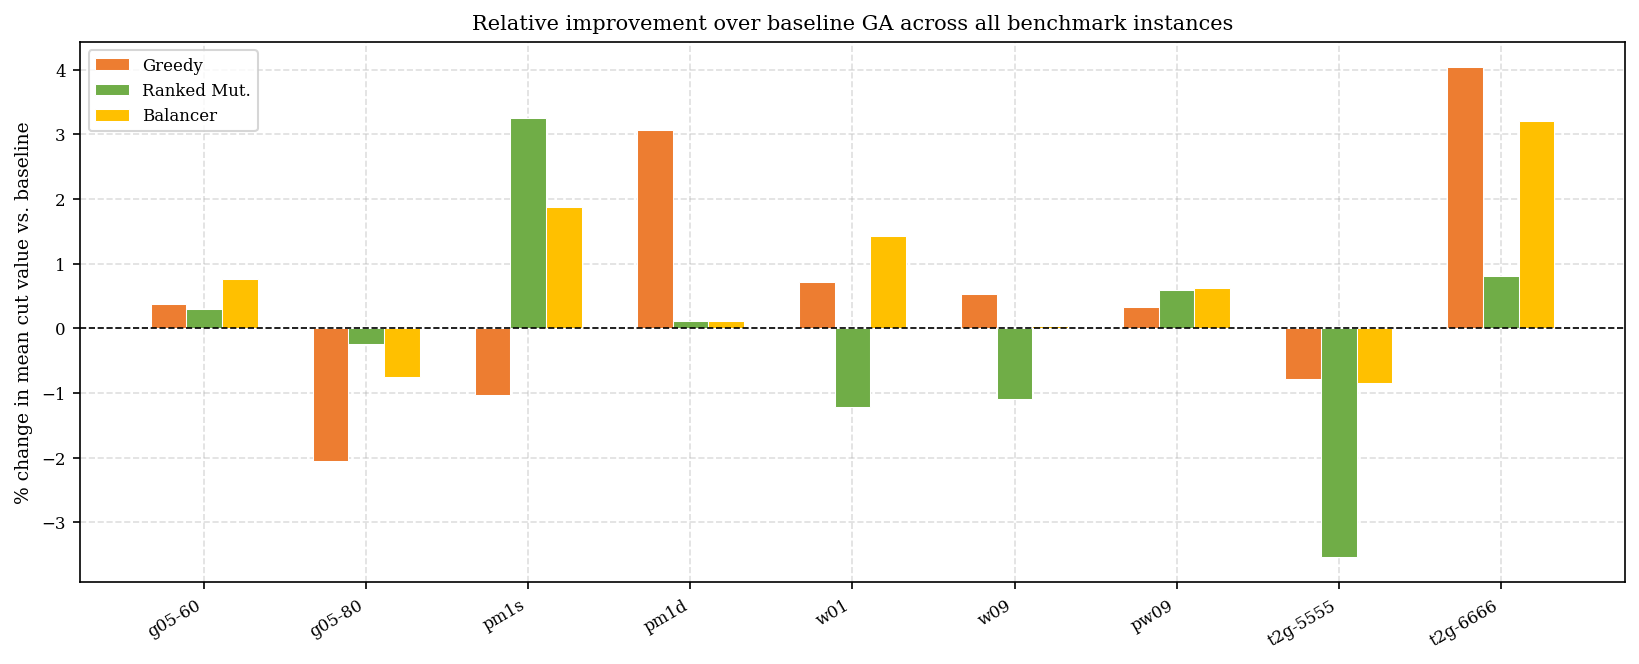
\includegraphics[width=\textwidth]{results/fig1_relative.png}
\caption{Relative change in mean cut value compared to the baseline GA
          (no heuristics), across all nine benchmark instances.
          Positive values indicate improvement over the baseline.
          Each bar is the mean over five independent runs.}
\label{fig:relative-improvement}
\end{figure}

\begin{figure}[H]
\centering
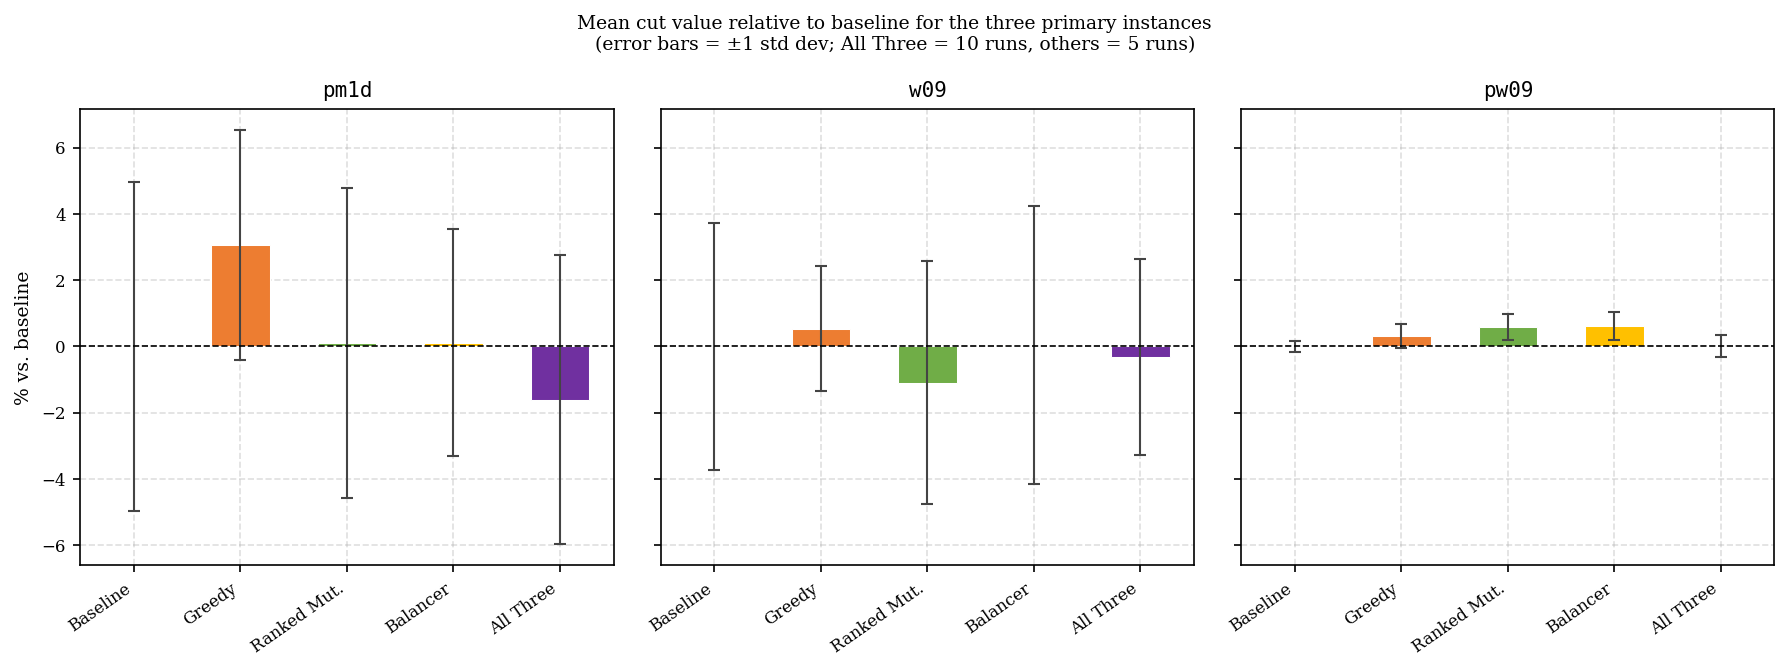
\includegraphics[width=\textwidth]{results/fig2_primary.png}
\caption{Mean cut value relative to the baseline (\%) for the three primary
          benchmark instances (\texttt{pm1d\_100.9}, \texttt{w09\_100.9},
          \texttt{pw09\_100.9}). Error bars show $\pm 1$ standard deviation
          over the repeated runs. The dashed line marks zero (baseline level).
          The \emph{All Three} bar corresponds to 10 runs; all others to 5.}
\label{fig:primary-instances}
\end{figure}

\begin{figure}[H]
\centering
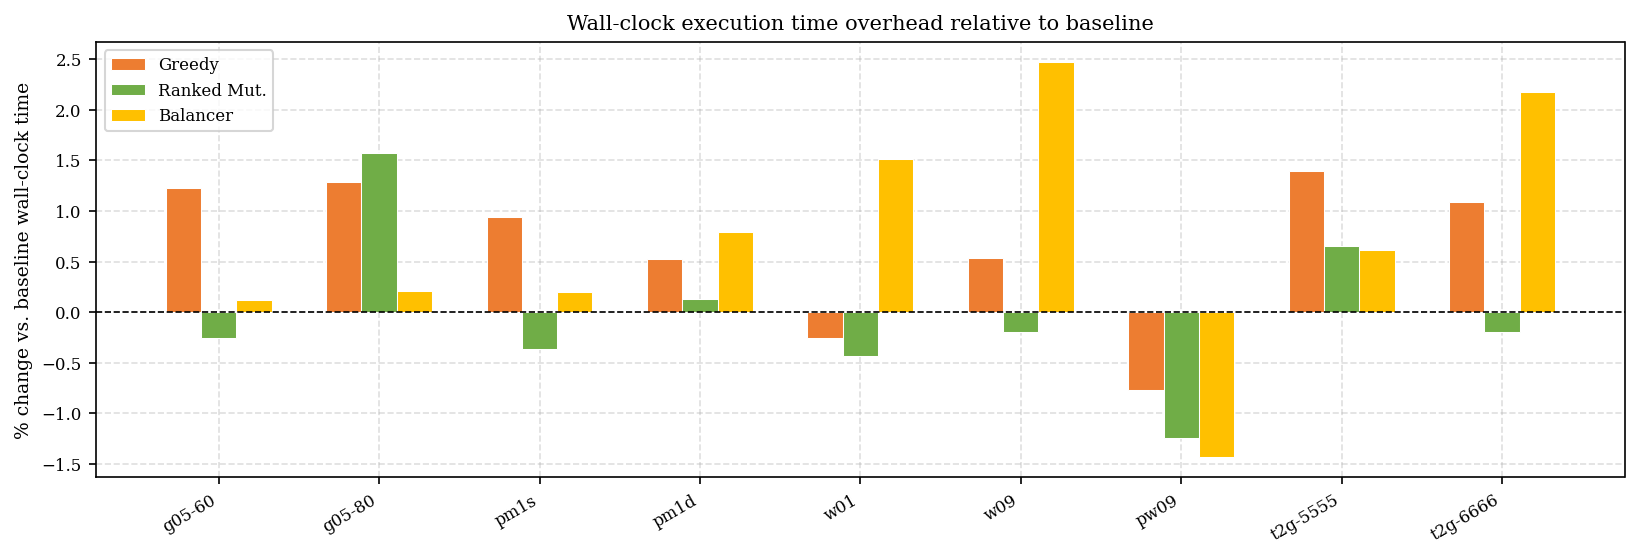
\includegraphics[width=\textwidth]{results/fig3_timing.png}
\caption{Wall-clock execution time of the evolutionary loop relative to
          the baseline (\%), per instance and heuristic.
          All deviations are within $\pm 3\%$, confirming that the
          heuristic operators introduce negligible computational overhead.}
\label{fig:timing}
\end{figure}

% ─────────────────────────────────────────────────────────────────────────────
\section{Analysis}
\label{sec:analysis}

\subsection{Heuristic effectiveness is instance-structure dependent}

The clearest pattern in the results (Figure~\ref{fig:relative-improvement}) is
that the benefit of each heuristic correlates strongly with the structural
properties of the instance rather than its size.
The greedy-by-node repair achieves its largest gains on the two instance
families with the most heterogeneous weight distributions: \texttt{pm1d} and
\texttt{t2g} (Tables~\ref{tab:results-pm1} and~\ref{tab:results-t2g}), where
the node ranking reliably identifies a small influential core.
On the unweighted \texttt{g05} family, where all edge weights are equal and the
ranking carries little information, the same heuristic is neutral or slightly
harmful (Table~\ref{tab:results-g05}).
This suggests a general principle: repair mechanisms that fix a subset of
vertices are only as useful as the ranking that selects them, and weight
heterogeneity is the primary driver of ranking quality.

\subsection{Balancer is the most robust single heuristic}

Across all nine instances the balancer produces no degradation larger than
$1\%$ and delivers the best or near-best single-heuristic result on five of
them (Figure~\ref{fig:relative-improvement}).
Unlike the greedy repair and ranked mutation — both of which depend on the
informativeness of the node ranking — the balancer acts on a structural
property of the partition that is instance-agnostic: excessive size asymmetry
correlates with poor cut value regardless of the graph topology.
Its consistently safe profile makes it the recommended default when no prior
knowledge about the instance family is available.

\subsection{Combining heuristics does not compound their benefits}

The three primary instances were tested with all heuristics active simultaneously
(Figure~\ref{fig:primary-instances}, Tables~\ref{tab:results-pm1}
and~\ref{tab:results-w}).
In no case does the combined configuration outperform the best individual
heuristic for that instance.
On \texttt{pm1d\_100.9} it is the worst-performing configuration ($-1.6\%$
below baseline), and on \texttt{w09\_100.9} and \texttt{pw09\_100.9} it
trails the single-heuristic leaders.
The likely cause is a diversity collapse: greedy repair pins the most
influential vertices to a fixed assignment, while ranked mutation simultaneously
suppresses variation on those same vertices, leaving the search with very
little freedom to escape local optima.
Enabling all three heuristics together therefore requires careful tuning and
is not advisable without instance-specific validation.

\subsection{Computational cost is negligible}

Figure~\ref{fig:timing} shows that all three heuristics introduce less than
$3\%$ wall-clock overhead relative to the baseline across every instance and
configuration tested.
Given that this variation is within normal run-to-run noise (the standard
deviations in the tables confirm similar variability in raw execution times),
the heuristics are effectively free in terms of computational budget.
Any observed differences in solution quality are therefore attributable
entirely to the operators themselves rather than to an expanded time allowance.

% ─────────────────────────────────────────────────────────────────────────────
\begin{thebibliography}{9}

\bibitem{biqmac}
A.~Wiegele,
\textit{Biq Mac Library: A Collection of Max-Cut and Quadratic 0-1 Programming
Instances of Medium Size},
Technical Report, Alpen-Adria-Universit\"{a}t Klagenfurt, 2007.
Available: \url{http://biqmac.aau.at/biqmaclib.html}

\bibitem{rudy}
G.~Rinaldi,
\textit{Rudy: A Graph Generator},
IASI-CNR, Rome.
Available: \url{http://www-user.tu-chemnitz.de/~helmberg/rudy.tar.gz}

\bibitem{liers}
F.~Liers,
\textit{Contributions to Determining Exact Ground-States of Ising Spin-Glasses
and to their Physics},
Ph.D.\ thesis, Universit\"{a}t zu K\"{o}ln, 2004.

\bibitem{dejong}
K.~A.~De~Jong,
\textit{An Analysis of the Behavior of a Class of Genetic Adaptive Systems},
Ph.D.\ thesis, University of Michigan, 1975.

\bibitem{goldberg}
D.~E.~Goldberg,
\textit{Genetic Algorithms in Search, Optimization, and Machine Learning},
Addison-Wesley, Reading, MA, 1989.

\end{thebibliography}

\end{document}   